\documentclass[tikz,10pt]{standalone}

\usepackage[utf8]{inputenc}
\usepackage{amsmath}
\usepackage{amssymb}
\usepackage{microtype}
% \usepackage[bibstyle=authoryear,citestyle=authoryear]{biblatex}
\usepackage{url}\urlstyle{tt}
\usepackage{xcolor}
\usepackage{listings}

\newcommand{\citell}[1]{{\color{gray}\citeauthor{#1} \citeyear{#1} -- \textit{\citetitle{#1}} \cite{#1}}}
\newtheorem{definition}{Definition}
\newtheorem{proposition}{Proposition}
\newtheorem{example}{Example}

\DeclareMathOperator*{\argmin}{arg\,min}


\newcommand\Lb[1]{\mathit{Lb}(#1)}
\newcommand\InvLb[1]{\mathit{Lb}^{-1}(#1)}
\newcommand\Lbs[1]{\mathit{Lbs}(#1)}
\def\eqdef{\stackrel{\text{df}}{=}}
\newcommand\Hd[1]{\mathit{Head}(#1)}
\newcommand\HH[1]{\mathit{H}(#1)}
\newcommand\BB[1]{\mathit{B}^+(#1)}
\newcommand\BBn[1]{\mathit{B}^-(#1)}
\newcommand\Bd[1]{\mathit{Body}(#1)}
\newcommand\Bdp[1]{\mathit{Body}^+(#1)}
\newcommand\Bdn[1]{\mathit{Body}^-(#1)}
\def\eqdef{\stackrel{\text{df}}{=}}


\newcommand{\Vd}{\ensuremath{V_{d}}} %Disjunctinive vertices
\newcommand{\Vc}{\ensuremath{V_{c}}} %Choice vertices
\newcommand{\Va}{\ensuremath{V_{a}}} %Atom vertices
\newcommand{\Epos}{\ensuremath{E_{+}}} %Positive edges
\newcommand{\Eneg}{\ensuremath{E_{-}}} %Negative edges

\newcommand{\program}{\ensuremath{P}} %Program
\newcommand{\pr}{\ensuremath{P_r}} %Program reference
\newcommand{\pf}{\ensuremath{P_f}} %Program foil


\newcommand{\pg}[1]{\ensuremath{G_{#1}}} %Program Graph
\newcommand{\mg}{\ensuremath{MG}} %Model Graph
\newcommand{\mgpi}[2]{\ensuremath{\mg_{#1}^{#2}}} %Model Graph for a given program and interpretation
\newcommand{\cg}[4]{\ensuremath{CM_{#1, #2}^{#3, #4}}} %Constrast Graph

\newcommand{\isdisj}[1]{\ensuremath{\mathit{dis}(#1)}} % Rule is a disjunction
\newcommand{\ischoice}[1]{\ensuremath{\mathit{choice}(#1)}} % Rule is a choice
\newcommand{\iscons}[1]{\ensuremath{\mathit{cons}(#1)}} % Rule is a constraint
\newcommand{\atoms}[1]{\ensuremath{\mathit{Atoms}(#1)}} % Set of atoms of a program

\newcommand{\lbl}[1]{\ensuremath{Lb(#1)}} %Literal

\newcommand{\removable}{\ensuremath{R_{\mathit{rem}}}} %Removable rules
\newcommand{\removed}{\ensuremath{R_{\mathit{rem}}^f}} %Removed rules
\newcommand{\addable}{\ensuremath{R_{\mathit{add}}}} %Addable rules
\newcommand{\added}{\ensuremath{R_{\mathit{add}}^f}} %Added rules

\newcommand{\pdiff}{\ensuremath{P{\mathit{diff}}}} %Program difference
\newcommand{\m}{\ensuremath{M}} %Model


\newcommand{\foils}{\ensuremath{\mathit{Foils}}} %Set of foils

\lstdefinelanguage{clingos}{%
  language=clingo,%
  basicstyle=\small\ttfamily%
}

\usepackage{tikz}
\usepackage{xcolor}
\usepackage{graphicx}
\usetikzlibrary{positioning}
\usetikzlibrary{fit}
\pgfdeclarelayer{background}
\pgfdeclarelayer{sections}
\pgfsetlayers{sections,background,main}
\definecolor{stylegreen}{HTML}{D7ECD9}
\definecolor{stylegreen}{HTML}{D7ECD9}
\definecolor{styleyellow}{HTML}{F6F6EB}
\definecolor{stylepurple}{HTML}{D5D6EA}
\definecolor{styleblue}{HTML}{D9EBF6}
\tikzset{
  node distance=6mm and 8mm,
  every node/.style={font=\scriptsize},
  element/.style={
    font=\scriptsize,
    fill=styleyellow,
    draw=black,
    % rounded corners,
    inner sep=3pt,
    align=center
  },
  encoding/.style={
    element,
    fill=stylepurple
  },
  input-file/.style={
    element,
    fill=stylegreen,
    align=left,
    inner sep=3pt
  },
  ctl/.style={
    element,
    double, rounded corners, font=\scriptsize, fill=gray!20, draw=black, inner sep=5pt, align=center
  },
  subsection/.style={
    draw=gray,
    rounded corners,
    fill=gray!10,
    inner sep=10pt
  },
  arrw/.style={
    -latex,
    font=\tiny
  },
  subarrw/.style={
    blue,
    densely dotted,
    -latex
  }
}

\begin{document}




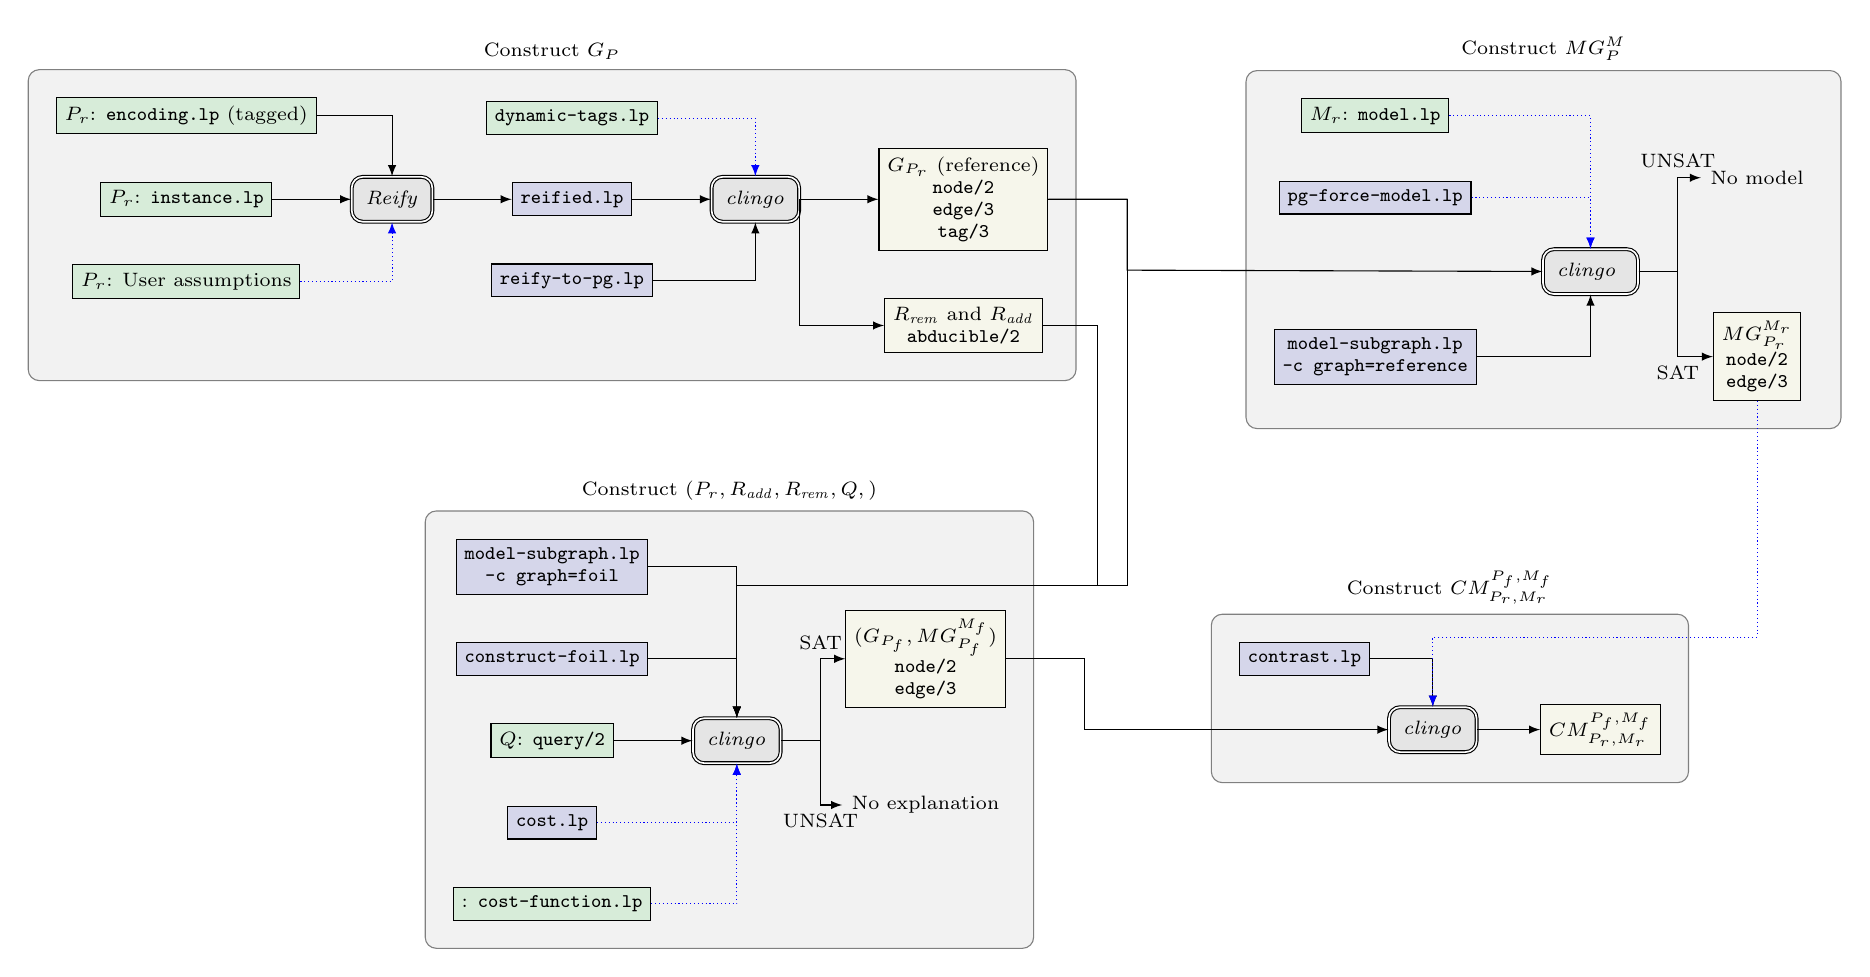
\begin{tikzpicture}


% ================= Construct PG =================
\node[input-file] (enc) {$\pr$: \texttt{encoding.lp} (tagged)};
\node[input-file, below=of enc] (inst) { $\pr$: \texttt{instance.lp}};
\node[input-file, below=of inst] (ass) { $\pr$: User assumptions};

% \begin{pgfonlayer}{background}
% \node[subsection, fit=(enc)(inst)(ass), label=above:{Program $\pr$}, fill=gray!20] (program) {};
% \end{pgfonlayer}


\node[ctl, right=10mm of inst] (meta-tools) {\textit{Reify}};

\node[encoding, right=10mm of meta-tools] (reify) {\texttt{reified.lp}};
\node[encoding, below=of reify] (reifypg) {\texttt{reify-to-pg.lp}};
\node[input-file, above=of reify] (dyn) {\texttt{dynamic-tags.lp}};

\node[ctl, right=10mm of reify] (constructpg) {\textit{clingo}};

\node[element, right=10mm of constructpg] (pg) {
  $\pg{\pr}$ (reference)\\ \texttt{node/2}\\ \texttt{edge/3}\\ \texttt{tag/3}
  };
  \node[element, below = of pg] (abd) {\removable\ and \addable\\\texttt{abducible/2}};


\draw[arrw] (enc) -| (meta-tools);
\draw[arrw] (inst) -- (meta-tools);
\draw[subarrw] (ass) -|  (meta-tools);
\draw[arrw] (meta-tools) -- (reify);
\draw[arrw] (reify.east) -- (constructpg);
\draw[arrw] (reifypg) -| (constructpg);
\draw[subarrw] (dyn) -| (constructpg);
\draw[arrw] (constructpg.east) -- (pg);
\draw[arrw] (constructpg.east) |- (abd.west);

\begin{pgfonlayer}{sections}
\node[subsection, fit=(enc)(inst)(ass)(reify)(reifypg)(dyn)(constructpg)(pg)(abd), label=above:{Construct \pg{P}}] (pgbox) {};
\end{pgfonlayer}

% ================= Reference Model (top right) =================
\node[input-file, right=125mm of enc] (model) {$\m_r$: \texttt{model.lp}};
\node[encoding, below=of model] (pgforce) {\texttt{pg-force-model.lp}};
\node[below=of pgforce] (ph){};
\node[encoding, below=of ph] (subg) {\texttt{model-subgraph.lp}\\\texttt{-c graph=reference}};

\node[ctl, right=20mm of ph] (constructref) {
  \textit{clingo}
};

\node[element, right=30mm of subg] (mgref) {$\mgpi{\pr}{\m_r}$ \\\texttt{node/2}\\\texttt{edge/3}};
\node[ above= 15mm of mgref] (unsat) {No model};

\draw[subarrw] (model.east) -| (constructref);
\draw[subarrw] (pgforce.east) -| (constructref);
\draw[arrw] (subg) -| (constructref);
\draw[arrw] (constructref.east) -- ++(0.5,0) |-  node[below]{SAT} (mgref);
\draw[arrw] (constructref.east) -- ++(0.5,0) |- node[above]{UNSAT} (unsat.west);

\begin{pgfonlayer}{sections}
\node[subsection, fit=(model)(pgforce)(subg)(constructref)(mgref)(unsat), label=above:{Construct $\mgpi{P}{\m}$}] (refbox) {};
\end{pgfonlayer}

% ================= Foils (bottom left) =================
\node[encoding, below=20mm of pgbox] (subgfoil) {\texttt{model-subgraph.lp}\\\texttt{-c graph=foil}};
\node[encoding, below=of subgfoil] (constructfoil) {\texttt{construct-foil.lp}};

\node[input-file, below=of constructfoil] (query) {$Q$: \texttt{query/2}};
\node[encoding, below=of query] (cost) {\texttt{cost.lp}};
\node[input-file, below=of cost] (costfn) {$\foilcost$: \texttt{cost-function.lp}};

\node[ctl, right=10mm of query] (clingofoil) {\textit{clingo}};

\node[element, right=25mm of constructfoil] (pgfoil) {$(\pg{\pf}, \mgpi{\pf}{\m_f})$ \\\texttt{node/2}\\\texttt{edge/3}};
\node[ below=10mm of pgfoil] (noex) {No explanation};
% \node[element, below=of pgfoil] (mgfoil) {$\mgpi{\pf}{\m_f}$ \\\texttt{node/2}\\\texttt{edge/3}};

\draw[arrw] (subgfoil) -| (clingofoil);
\draw[arrw] (constructfoil) -| (clingofoil);
\draw[arrw] (query) -- (clingofoil);
\draw[subarrw] (cost) -| (clingofoil);
\draw[subarrw] (costfn) -| (clingofoil);
\draw[arrw] (clingofoil.east) -- ++(0.5,0) |- node[above]{SAT} (pgfoil);
\draw[arrw] (clingofoil.east) -- ++(0.5,0) |- node[below]{UNSAT} (noex.west);

% \draw[arrw] (clingofoil) -- (mgfoil);

\begin{pgfonlayer}{sections}
\node[subsection, fit=(subgfoil)(constructfoil)(query)(cost)(costfn)(clingofoil)(pgfoil), label=above:{Construct $\bestfoils(\pr, \addable, \removable, Q, \foilcost)$}] (foilbox) {};
\end{pgfonlayer}

% ================= Contrastive (bottom right) =================
\node[ctl, right=45mm of foilbox] (contrast) {\textit{clingo}};
\node[encoding, right= 75mm of constructfoil] (contrastenc) {\texttt{contrast.lp}};
\node[element, right=8mm of contrast] (cg) {\cg{\pr}{\m_r}{\pf}{\m_f}};

\draw[arrw] (contrastenc) -| (contrast);

\begin{pgfonlayer}{sections}
\node[subsection, fit=(contrastenc)(contrast)(cg),  label=above:{Construct \cg{\pr}{\m_r}{\pf}{\m_f}}] (contrastbox) {};
\end{pgfonlayer}


\draw[subarrw] (mgref.south) -- ++(0,-3) -| (contrast);
\draw[arrw] (pgfoil.east) -- ++(1,0) |- (contrast);
\draw[arrw] (contrast) -- (cg);
\draw[arrw] (pg.east) -- ++(1,0) -- ++(0,-0.9) -- (constructref);
\draw[arrw] (pg.east) -- ++(1,0) -- ++(0,-4.9) -| (clingofoil.north);
\draw[arrw] (abd.east) -- ++(0.7,0) -- ++(0,-3.3) -| (clingofoil.north);
\end{tikzpicture}


\end{document}
